\addcontentsline{toc}{chapter}{\textsl{Bl\aa stjernehav Familie- \& Dukketeater}}
\chapter*{ \textsl{\textbf{BL\AA STJERNEHAV  \\ FAMILIE- \& DUKKETEATER}}}

\label{psh}

\vspace{1cm}

{\Large \textbf{Presentation}}

\bigskip
\bigskip

The project \textsl{Bl\aa stjernehav Familie- \& Dukketeater} proposes two performative modes: 
\begin{enumerate}
\item The play itself -- once a week for instance -- where the kids play in the boat-carrousel with interactive quadrophonic soundscape for their families and audience;
\item and the stage of the play as a fjord-landscape `3D-tableau' installation with experimental sonic sculpture.
\end{enumerate}

\bigskip

The following documentation shows a possible play, and it is best to visualize it as a sketch, showing how the theatre was played and exhibited in Troms\o{} Kunstforening from the 14th of August to the 11th of October 2020. 

\bigskip

\begin{figure}[h]
		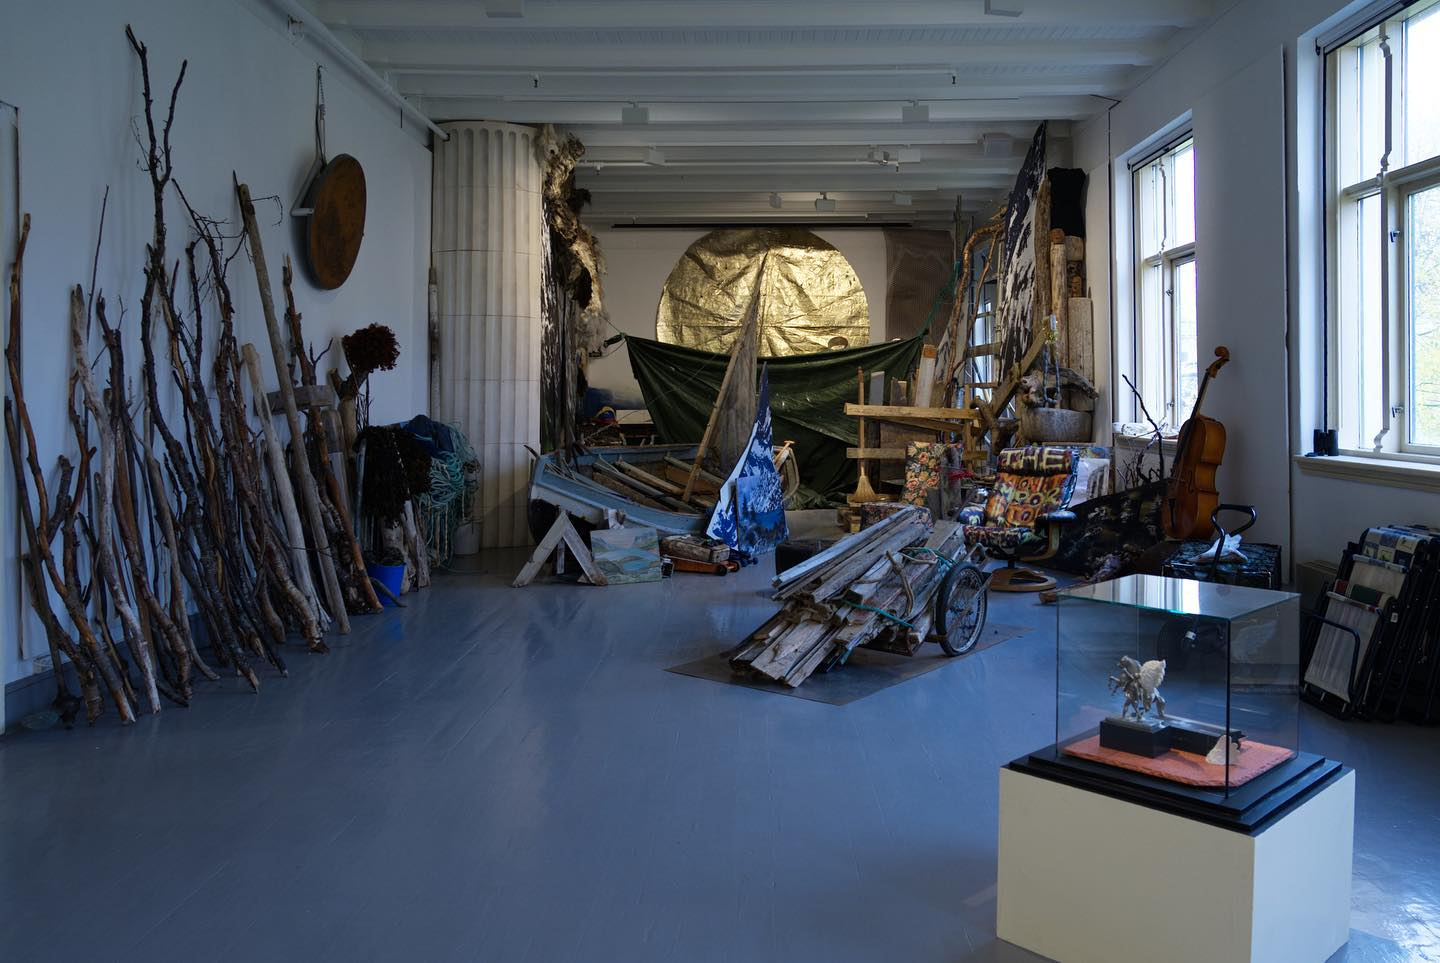
\includegraphics[width=\textwidth]{mp/img/img1}
		%\caption{}
		\label{sh}
\end{figure}

\newpage 

\noindent {\Large \textsl{\textbf{Selenes Havbrev}}}

\bigskip

\noindent \textbf{\textsl{Ly til fantasi og fellesskap}} 14.08.2020 -- 11.10.2020 \vspace{1mm} \\ 
$\rightarrow$ \href{http://www.tromsokunstforening.no/default.asp?cmd=100&UtsID=200}{\texttt{\footnotesize http://www.tromsokunstforening.no/Ly\_til\_fantasi\_og\_fellesskap}} 

\bigskip

[ ... ] \textsl{Forestillingen `Selenes havbrev' og `Selenes sang' er skrevet av Ane Elene Johansen, og maleriene er laget av Asbj\o{}rn Hillingseter L\o{}yning. Yann Ics har komponert musikk og lydbilde, og scenografien er laget av H\aa vard Arnhoff som ogs\aa  er initiativtakeren bak teateret.}

\smallskip

\begin{figure}[h]
	\begin{center}
		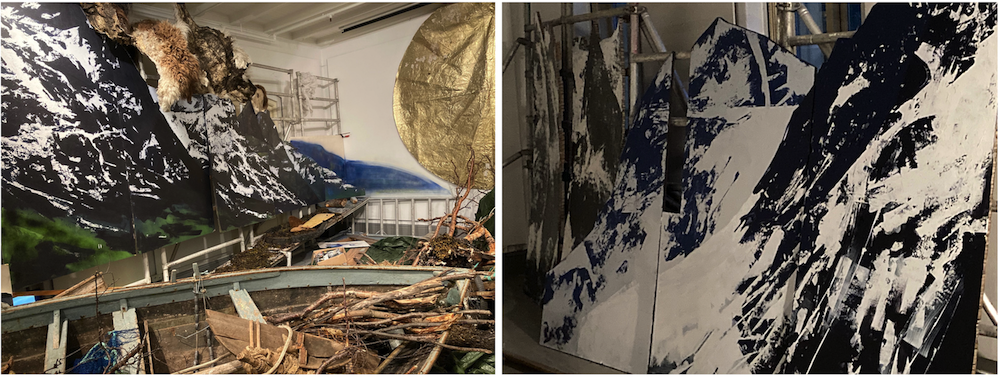
\includegraphics[width=0.99\textwidth]{mp/img/img2}
		%\caption{}
		\label{sh}
	\end{center}
\end{figure}

\begin{enumerate}
\item \textbf{The play} $\rightarrow$ pages \pageref{shtp1} to \pageref{shtp2}. 
\begin{figure}[H]
\hfill 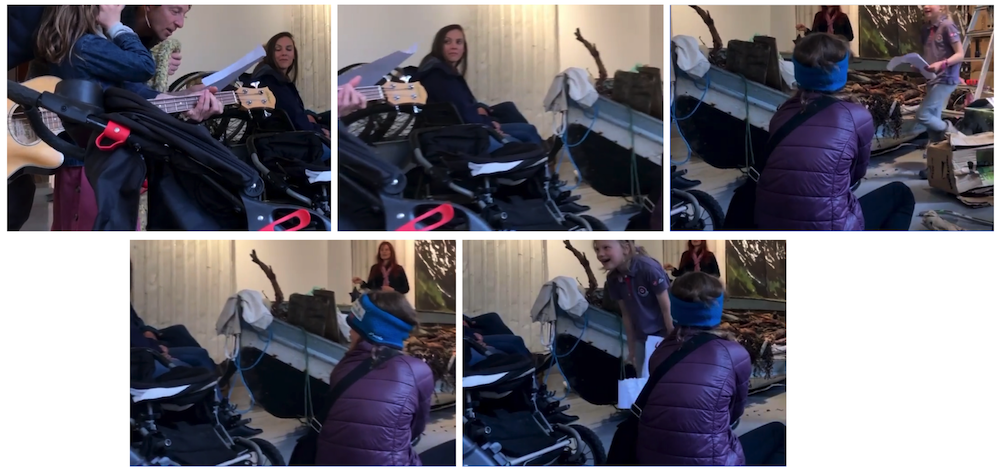
\includegraphics[width=0.92\textwidth]{mp/img/img3}
\end{figure} 
\item \textbf{On the side} \\ \\ 
$\rightarrow$ Study of a sonic sculpture on two recycled corrugated sheets as installation from the 22nd of August to the 29th of August 2020 in Troms\o{} Kunstforening.
\begin{figure}[H]
\hfill 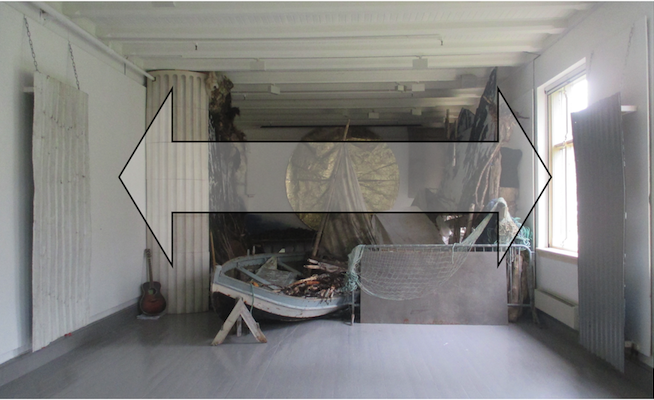
\includegraphics[width=0.92\textwidth]{mp/img/img4}
\end{figure}
This installation performed the score of the second guitar of the composition \textsl{Selenes Havbrev} [ $\rightarrow$ page \pageref{sh} ] with the digital wave guide physical model of a bowed instrument plus improvised composition. \\ \\
$\rightarrow$ Surrealistic sound installation performed in Troms\o{} Kunstforening between the 25th of September and the 11th of October 2020. 
\begin{figure}[H]
\hfill 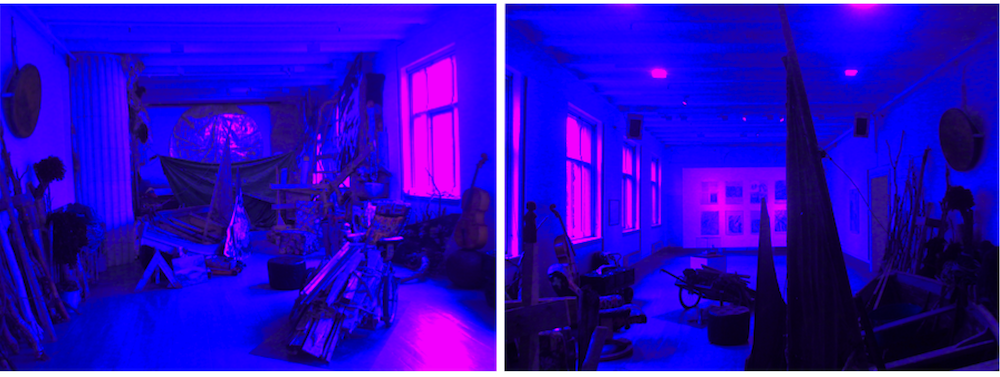
\includegraphics[width=0.92\textwidth]{mp/img/img5}
\end{figure}
Experimenting different physical models -- as a bowed instrument and the acoustics of tube models -- using respectively a cello and a parabolic antenna, as part of a `post-apocalyptic' ambient quadraphonic soundscape which the latest can be depicted as a  `walking on the \textit{Ersfjordbotn} beach'.
\end{enumerate}

\begin{figure}[htp]
	\begin{center}
		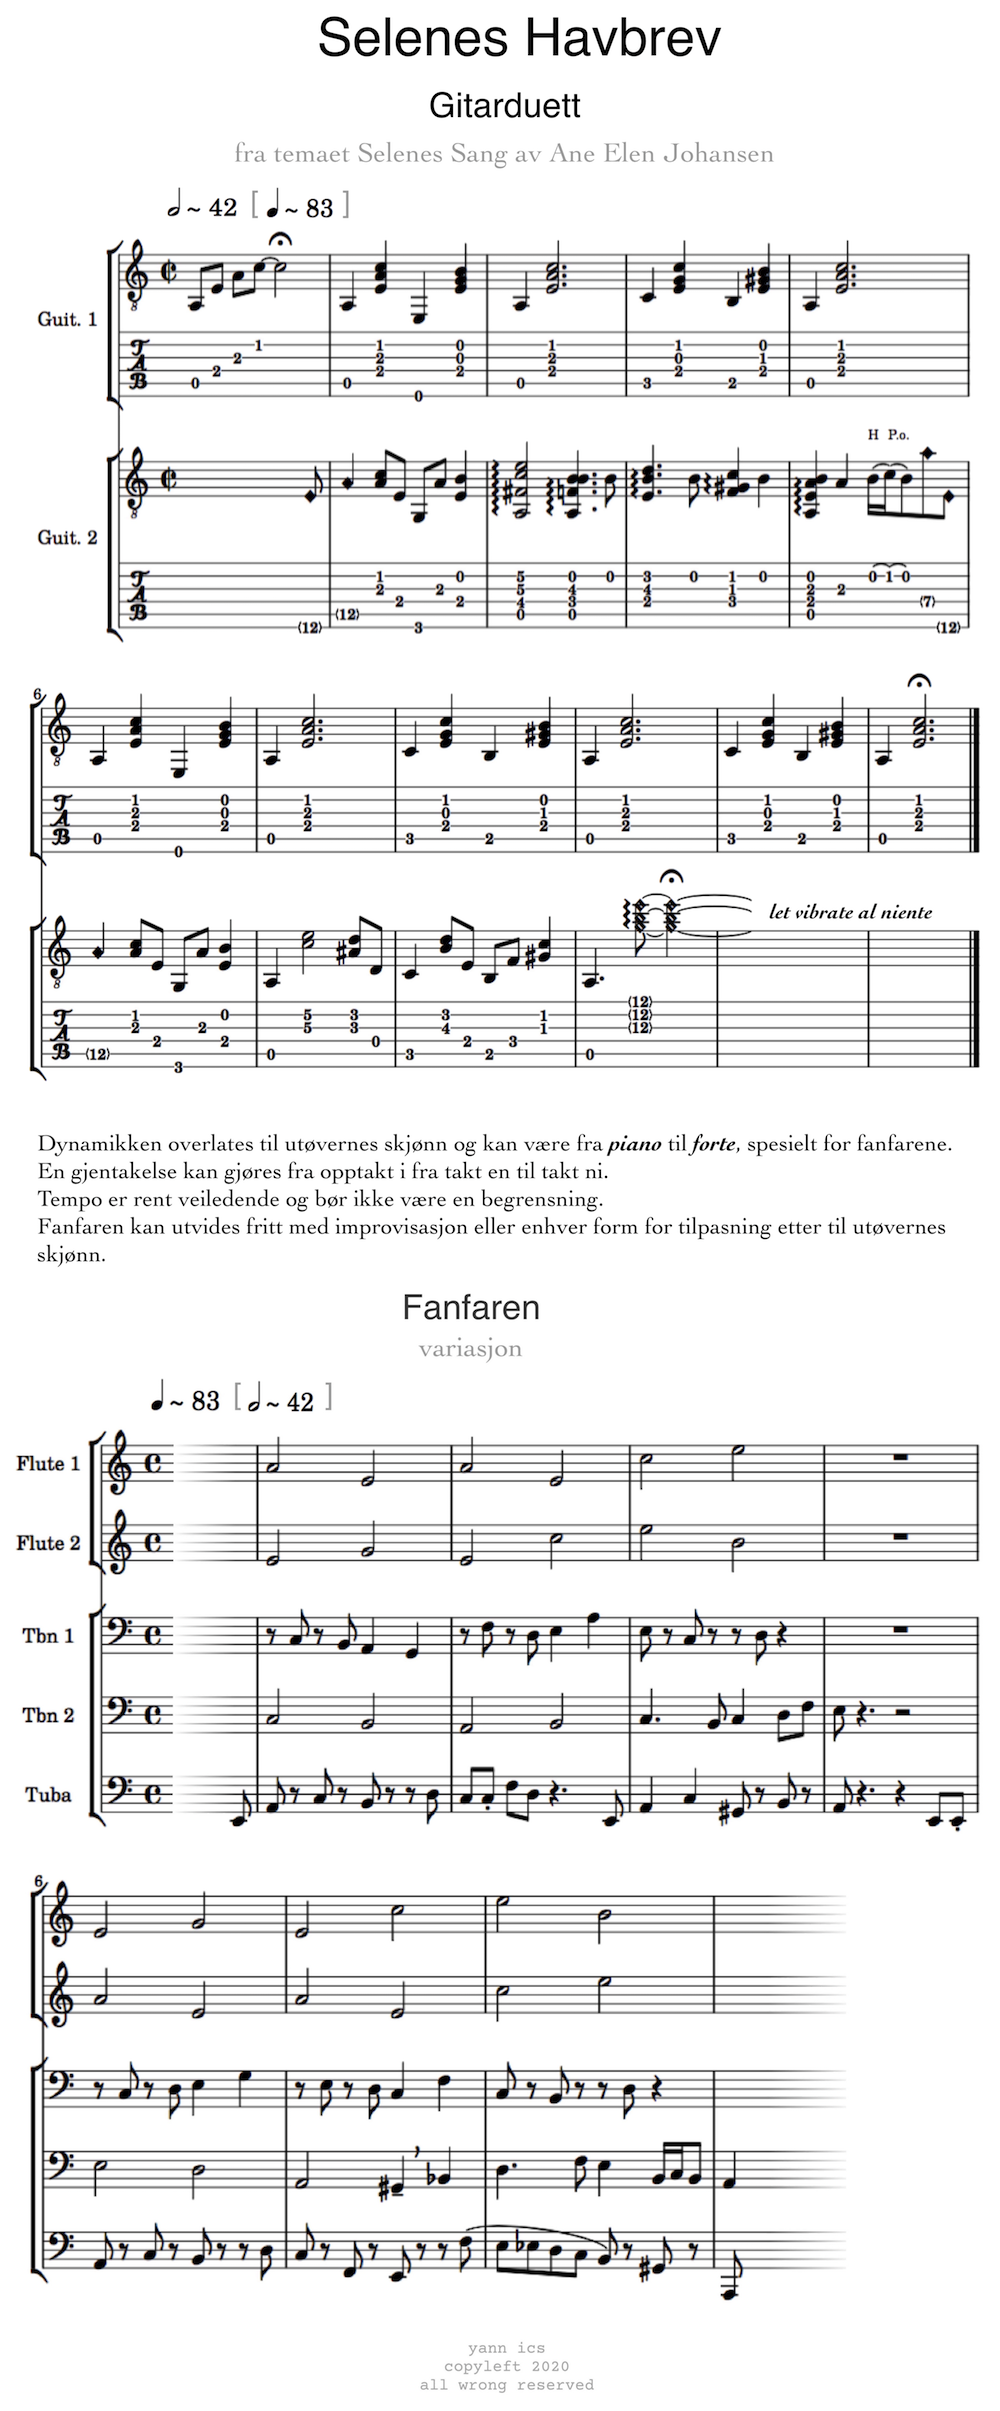
\includegraphics[width=0.65\textwidth]{mp/img/img6}
		%\caption{}
		\label{sh}
	\end{center}
\end{figure}

\bigskip
\bigskip
\bigskip
\bigskip

\begin{center}
  \LARGE\bfseries{\textsl{Selenes Havbrev}}
\end{center}
\label{shtp1}

\bigskip
\bigskip
{\small 
\hfill \textbf{av Ane E. Johansen.}

\bigskip 
 \bigskip

\noindent \textit{\color{gray} En fjord. Fj\ae re. En b\aa t.}

\noindent \textit{\color{gray} Ei jente kjem fram av b\aa ten. Kravlende ut, som ei forsiktig krabbe. Stiller seg fram p\aa  scenen og proklamerer:}

\begin{description}
\item[Marikkel]: I natt hadde \ae  en dr\o{}m. Tre lysende stjerner s\aa  vi p\aa  v\aa rsolas himmel i natt. Det betyr at selene kjem med Havbrevet. \AE  og mi s\o{}ster skal st\aa  klar og ta imot! 
\item[Sardina]: Han pappa sover inne i huset enda. Han treng s\o{}vnen sin no, for ho mamma har kommet til himmelen og han pappa er fryktelig lei seg.
\end{description}

\noindent \textit{\color{gray} Samtidig som Sardina sier dette, g\aa r Marikkel og setter seg i b\aa ten og venter. Hun tar p\aa  seg en sydvest og begynner \aa  ordne til noe fiskesaker.}

\noindent \textit{\color{gray} Sola glinser i horisonten. Lyset er vidunderlig. Det skinner p\aa  fjellsidene.}

\begin{description}
\item[Sardina]: Marikkel, har du sjekka nisa om den e klar?
\item[Marikkel]: Jada, vi har alt p\aa  stell. Trur du vi ska fare med \'{e}n gang?
\item[Sardina]: Best \aa  ikkje vente for lenge. \AE  dr\o{}mte at vi m\aa tte v\ae re klar p\aa  stiganes flo!
\item[Marikkel]: Tenk at vi har dr\o{}mt det samme! Men med floa kjem vinden..
\item[Sardina]: Det e no eller aldri!
\end{description}

\noindent \textit{\color{gray} Sardina skyver b\aa ten ut mot vannet og hiver seg oppi b\aa ten. De tar fram \aa rene og begynner \aa  ro. De ror og ror seg lengre og lengre utover fjorden. Med ett bl\aa ser det opp til storm.}

\begin{description}
\item[Marikkel]: Det bl\aa ser opp til storm! Vi m\aa  snu! 
\end{description}

\noindent \textit{\color{gray} De f\aa r vansker med \aa  holde \aa rene, og de mister ei \aa re i b\o{}lgene.}

\begin{description}
\item[Sardina]: \AA  nei, jeg mista \aa ra! Hjelp meg, f\aa r du tak i den? 
\item[Marikkel]: Nei, den forsvinner!
\end{description}

\noindent \textit{\color{gray} Sardina b\o{}yer seg over ripa og pr\o{}ver \aa  f\aa  tak i den, og plutselig faller hun ned i vannet.}

\begin{description}
\item[Sardina]:  \textit{\color{gray} (roper)} Marikkel! 
\end{description}

\noindent \textit{\color{gray} Uv\ae ret fortsetter, og Sardina holder p\aa  \aa  drukne. Marikkel fors\o{}ker \aa  n\aa  henne med den ene \aa ra si. Sardina forsvinner lengre og lengre bort fra b\aa ten. Marikkel ror etter og pr\o{}ver \aa  n\aa  henne igjen. Men det er sterke b\o{}lger og hardt \aa  ro.}

\begin{description}
\item[Marikkel]: Ta \aa ra! Ta \aa ra!
\end{description}

\noindent \textit{\color{gray} Sardina griper i panikk rundt \aa ra og Marikkel greier \aa  f\aa  henne om bord i b\aa ten igjen. Sardina klemmer i ett hardt grep rundt Marikkel og da hoster Marikkel og v\aa kner til liv.}

\begin{description}
\item[Sardina]:  \textit{\color{gray} (hoster)} Hvor kom det uv\ae ret fra? 
\item[Marikkel]: Flovinden, Sardina! \AE  sa det til d\ae ! Vi m\aa  bare fortsette \aa  ro. Vi er kommet s\aa  langt no, vi vil ikkje klare \aa  ro mot b\o{}lgan inn til land igjen. 
\end{description}

\noindent \textit{\color{gray} De ror med \aa rene som er igjen gjennom uv\ae ret.}

\begin{description}
\item[Marikkel]: Her kan vi g\aa  i land! 
\end{description}

\noindent \textit{\color{gray} De ror seg i land ved ei bukt og drar b\aa ten i land og fort\o{}yer den. Sakte gir uv\ae ret seg og det blir blank stilla hav.}

\begin{description}
\item[Sardina]: Se, Marikkel!  \textit{\color{gray} (Peker p\aa  himmelen)} Tre stjerner p\aa  v\aa rsolas himmel. Det var hit vi skulle, uv\ae ret ledet oss hit!
\item[Marikkel]: Ja, tenk at det blei s\aa nn!
\item[Marikkel]: Da er tida inne.  \textit{\color{gray} (En liten pause til ettertanke)} 
\end{description}

\noindent \textit{\color{gray} Sola lyser fram igjen og det glitrende landskapet trer fram i lyset.}

\noindent \textit{\color{gray} Plutselig h\o{}rer de noe i havet som fanger oppmerksomheten deres. Tre seler kjem sv\o{}mmende mot dem.}

\begin{description}
\item[Sardina]: Der kjem selene  \textit{\color{gray} (sier det andektig)}. 
\end{description}

\noindent \textit{\color{gray} Selene holder et tau i munnene sine. Den ene til den andre. Tauet er spunnet av tang. I tauet henger det ei lita kiste. Selene kjem i land i fj\ae rsteiene og danser p\aa  sitt fornurlige vis mot jentene. Selene synger:}

\begin{description}
\item[Selene]: \textit{\color{gray} (Selenes Sang)} 
\end{description}

\begin{quote}
\begin{guitar}
\smallskip
I [\color{gray} Am]natt har vi [\color{gray} Em]spunnet ei vi[\color{gray} Am]se\smallskip
Tre [\color{gray} C]stjerner i v\aa r[\color{gray} E]solelyset[\color{gray} Am]\smallskip
V\aa rt [\color{gray} Am]brev kjem fra ha[\color{gray} Em]vets kiste[\color{gray} Am]\smallskip
[\color{gray} C]Aldri m\aa  vi glem[\color{gray} E]me eller miste.[\color{gray} Am]

\end{guitar}
\end{quote}

\noindent \textit{\color{gray} Selene gir kista til jentene. Jentene takker og bukker.} 

\begin{description}
\item[Marikkel]: Takk skal dere ha. 
\item[Sardina]: Hvordan kan en dr\o{}m bli sann? 
\item[Selene]: \textit{\color{gray} (sier i kor)} Dr\o{}mte dere hva dere skulle gj\o{}re med brevet vi har kommet med? 
\item[Marikkel]: \textit{\color{gray} (Forundret)} Nei, her stopper dr\o{}mmen. 
\end{description}

\noindent \textit{\color{gray} Jentene ser p\aa  hverandre.}

\begin{description}
\item[Selene]: \textit{\color{gray} (sier i kor)} Aldri m\aa  vi glemme eller miste, dr\o{}mmen om bl\aa stjernehav. Ta dette brevet og gi det til den dere holder mest av. 
\end{description}

\noindent \textit{\color{gray} S\aa  forsvinner selene ut i havets dyp.}

\noindent \textit{\color{gray} Jentene st\aa r igjen med den lille kista.} 

\begin{description}
\item[Marikkel]: Hva mente selene? Aldri m\aa  vi glemme eller miste, dr\o{}mmen om bl\aa stjernehav. Ta dette brevet og gi det til den dere holder mest av \textit{\color{gray} (repeterer etter selene)}. 
\item[Sardina]: Nei, si det. Kanskje vi m\aa  gi det til den vi stoler mest p\aa  i hele verden? 
\end{description}

\noindent \textit{\color{gray} De \aa pner kista. Der ligger det et bl\aa tt hjerte av glass. Marikkel tar hjertet varsomt ut av kista og holder det opp mot lyset.}

\begin{description}
\item[Marikkel]: Se, kor vakkert!
\item[Sardina]: Ja, se kor det glinse og banke! Et bl\aa tt hjerte!
\end{description}

\noindent \textit{\color{gray} De studerer hjertet. Ser det fra alle vinkler, beundrer det.}

\begin{description}
\item[Marikkel]: Vi tar det med hjem til han pappa, s\aa  blir han glad.
\item[Sardina]: Ja, det gj\o{}r vi!
\end{description}

\noindent \textit{\color{gray} De hiver seg i b\aa ten, men oppdager at den begynner \aa  ta inn vatn.}

\begin{description}
\item[Marikkel]: Se, s\o{}ster, b\aa ten begynner \aa  ta inn vann!
\item[Sardina]: Vi kan ikkje komme oss hjem over fjellene!
\end{description}

\noindent \textit{\color{gray} De ser seg omkring p\aa  fjellene rundt. Og stirrer ut i havet.}

\begin{description}
\item[Marikkel]: \textit{\color{gray} (Sier rolig og bestemt)} Da er vi n\o{}dt til \aa  ro hjem. 
\end{description}

\noindent \textit{\color{gray} De setter b\aa ten i havet og begynner \aa  ro. Et alvor legger seg over stemninga. De skj\o{}nner at dette kommer til \aa  bli farlig.} 

\begin{description}
\item[Sardina]: Vi f\aa r ro s\aa  st\o{}dig og fort vi bare kan. 
\end{description}

\noindent \textit{\color{gray} De kommer inn i en god rytme. N\aa  og da tar Marikkel \o{}sekaret og hiver ut vann fra b\aa ten. De ror og de ror. Jo lengre de ror, jo mer m\aa  de bruke \o{}sekaret. De ser bakover for \aa  se hvor langt de har igjen.}

\begin{description}
\item[Marikkel]: \AA , no m\aa  det ikkje v\ae re langt igjen! B\aa ten tar inn mer og mere vann! 
\item[Sardina]: Vi m\aa  bare holde ut! \AE  h\aa pe vi rekk det!
\item[Marikkel]: \textit{\color{gray} (ser seg bakover og studerer huset og naustet der de bor)} E det ikkje han pappa som st\aa r i fj\ae rsteinan der borte?
\item[Sardina]: Jo, det e det! Pappa!
\end{description}

\noindent \textit{\color{gray} Mannen i fj\ae ra vinker med begge armene, og roper tilbake.}

\begin{description}
\item[Pappa]: Sardina og Marikkel!
\end{description}

\noindent \textit{\color{gray} Mannen hiver seg i en b\aa t og ror i m\o{}te med dem. N\aa r b\aa tene m\o{}tes, klyver Sardina og Marikkel i pappas b\aa t, og han fort\o{}yer den fast i sin egen.}

\begin{description}
\item[Sardina og Marikkel]: Pappa! 
\end{description}

\noindent \textit{\color{gray} De gir hverandre en stor klem.}

\begin{description}
\item[Pappa]: Jentene mine. E dokker ute p\aa  havet no, med den gamle b\aa ten! Den l\ae k, jo! Og s\aa  tidlig p\aa  morran mens \ae  s\o{}v. Nei og nei, \ae  har v\ae rt s\aa  redd f\o{}rr kor dokker va! 
\item[Marikkel]: Pappa, vi, unnskyld! Vi hadde en dr\o{}m om at vi m\aa tte p\aa  havet, og s\aa  fikk vi ikkje sove. Pappa, vi --
\item[Sardina]: \textit{\color{gray} (avbryter)} Pappa, vi har opplevd s\aa  mye! Vi har m\o{}tt sela og, vi mesta ei \aa ra, det va s\aa  mye b\o{}lga, og selan ga oss nokka vi ville gje tel d\ae -
\item[Pappa]: Har selan gjedd dokker nokka, nei, ka dokker f\o{}rtell- 
\item[Marikkel og Sardina]: \textit{\color{gray} (i kor, andektig)} Aldri m\aa  vi glemme eller miste, dr\o{}mmen om bl\aa stjernehav. Ta dette brevet og gi det til den dere holder mest av. 
\end{description}

\noindent \textit{\color{gray} Sardina og Marikkel \aa pner kista av skjell og gir det bl\aa  hjertet til pappa.}

\begin{description}
\item[Pappa]: \textit{\color{gray} (utbryter)} \AA h...! Mammas gamle smykkestein! Kordan...?
\end{description}

\noindent \textit{\color{gray} Pappa holder det varsomt og stryker det bl\aa  hjertet forsiktig. T\aa rene renner nedover kinnene hans.}

\begin{description}
\item[Marikkel]: E det mamma sin smykkestein- ! 
\end{description}

\noindent \textit{\color{gray} Marikkel og Sardina ser p\aa  hverandre. De alle ser p\aa  hverandre sp\o{}rrende.} 

\noindent \textit{\color{gray} Med ett h\o{}rer de en fanfare i horisonten. Det er melodien som selene sang. De klemmer hverandre og smiler. Lyset gnistrer og blender.}
\color{black}
\label{shtp2}}

\bigskip
\bigskip
\bigskip

\begin{center} 
{\color{lightgray}\textsf{\small Selenes Havbrev}}
\bigskip

\textbf{\textsl{Post Scriptum}}

{\color{gray}{\scriptsize  \texttt{Copyleft \textcopyleft \, 2020 Yann Ics - All Wrongs Reserved.}}}
 \end{center} 
 
\bigskip 

\begin{figure}[h!]
		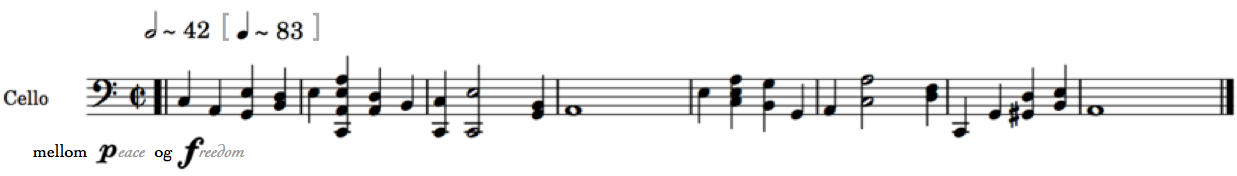
\includegraphics[width=1\textwidth]{mp/img/img7}
		%\caption{}
		\label{ps}
\end{figure}
